\chapter{Reference manuals for the \why tools}
\label{chap:manpages}

\section{Compilation, Installation}
\label{sec:install}

Compilation of \why must start with a configuration phase which is run as
\begin{verbatim}
./configure
\end{verbatim}
This analyzes your current configuration and checks if requirements hold.
Compilation requires:
\begin{itemize}
\item The Objective Caml compiler, version 3.10 or higher. It is
  available as a binary package for most Unix distributions. For
  Debian-based Linux distributions, you can install the packages
\begin{verbatim}
ocaml ocaml-native-compilers
\end{verbatim}
It is also installable from sources, downloadable from the site
\url{http://caml.inria.fr/ocaml/}
\end{itemize}

\noindent
For some tools, additional OCaml libraries are needed:
\begin{itemize}
\item For the IDE: the Lablgtk2 library for OCaml bindings of the gtk2
  graphical library. For Debian-based Linux distributions, you can
  install the packages
\begin{verbatim}
liblablgtk2-ocaml-dev liblablgtksourceview2-ocaml-dev
\end{verbatim}
It is also installable from sources, available from the site
\url{http://wwwfun.kurims.kyoto-u.ac.jp/soft/olabl/lablgtk.html}

\item For \texttt{why3bench}: The OCaml bindings of the sqlite3 library.
For Debian-based Linux distributions, you can install the package
\begin{verbatim}
libsqlite3-ocaml-dev
\end{verbatim}
It is also installable from sources, available from the site
\url{http://ocaml.info/home/ocaml_sources.html#ocaml-sqlite3}
\end{itemize}

When configuration is finished, you can compile \why.
\begin{verbatim}
make
\end{verbatim}
Installation is performed (as super-user if needed) using
\begin{verbatim}
make install
\end{verbatim}
Installation can be tested as follows: 
\begin{enumerate}
\item install some external provers (see~Section\ref{provers} below)
\item run \verb|why3config --detect|
\item run some examples from the distribution, \emph{e.g.} you should
obtain the following:
\begin{verbatim}
$ cd examples
$ why3replayer scottish-private-club
Info: found directory 'scottish-private-club' for the project
Opening session...[Xml warning] prolog ignored
[Reload] file '../scottish-private-club.why'
[Reload] theory 'ScottishClubProblem'
 done
Progress: 4/4
 1/1
Everything OK.
$ why3replayer programs/same_fringe
Info: found directory 'programs/same_fringe' for the project
Opening session...[Xml warning] prolog ignored
[Reload] file '../same_fringe.mlw'
[Reload] theory 'WP SameFringe'
[Reload] transformation split_goal for goal WP_parameter enum 
[Reload] transformation split_goal for goal WP_parameter eq_enum 
 done
Progress: 12/12
 3/3
Everything OK.
\end{verbatim}
\end{enumerate}

\subsection{Local use, without installation}

It is not mandatory to install \why into system directories.
\why can be configured and compiled for local use as follows:
\begin{verbatim}
./configure --enable-local
make
\end{verbatim}
The \why executables are then available in the subdirectory \texttt{bin/}.

\subsection{Installation of the \why library}
\label{sec:installlib}

By default, the \why library is not installed. It can be installed using
\begin{verbatim}
make byte opt
make install_lib
\end{verbatim}

\section{Installation of external provers}
\label{provers}

\why can use a wide range of external theorem provers. These need to
be installed separately, and then \why needs to be configured to use
them. There is no need to install these provers before compiling and
installing Why.

For installation of external provers, please look at the Why provers
tips page \url{http://why.lri.fr/provers.en.html}.

For configuring \why to use the provers, follow instructions given in
Section~\ref{sec:why3config}.

\section{The \texttt{why3config} command-line tool}
\label{sec:why3config}

\why must be configured to access external provers. Typically, this is done
by running
%%either
the command line tool \texttt{why3config}.
%%or using the menu
%%\begin{verbatim}
%%File/Detect provers
%%\end{verbatim}
%%of the IDE.
This must be redone each time a new prover is installed.

The provers which \why attempts to detect are described in
the readable configuration file \texttt{provers-detection-data.conf}
of the \why data directory (\eg{}
\texttt{/usr/local/share/why3}). Advanced users may try to modify this
file to add support for detection of other provers. (In that case,
please consider submitting a new prover configuration on the bug
tracking system).

The result of provers detection is stored in the user's
configuration file (\verb+~/.why3.conf+ or, in the case of local
installation, \verb+why3.conf+ in Why3 sources top directory). This file
is also human-readable, and advanced users may modify it in order to
experiment with different ways of calling provers, \eg{} different
versions of the same prover, or with different options.

The provers which are typically looked for are
\begin{itemize}
\item Alt-Ergo~\cite{conchon08smt,ergo}: \url{http://alt-ergo.lri.fr}
\item CVC3~\cite{BarTin-CAV-07}: \url{http://cs.nyu.edu/acsys/cvc3/}
\item Coq~\cite{CoqArt}: \url{http://coq.inria.fr}
\item Eprover~\cite{schulz04ijcar}: \url{http://www4.informatik.tu-muenchen.de/~schulz/WORK/eprover.html}
\item Gappa~\cite{melquiond08rnc}: \url{http://gappa.gforge.inria.fr/}
\item Simplify~\cite{simplify05}: \url{http://secure.ucd.ie/products/opensource/Simplify/}
\item Spass: \url{http://www.spass-prover.org/}
\item Vampire: \url{http://www.voronkov.com/vampire.cgi}
\item VeriT: \url{http://www.verit-solver.org/}
\item Yices~\cite{DM06}: \url{http://yices.csl.sri.com/}, only versions 1.xx since versions 2.xx do not support quantifiers
\item Z3~\cite{z3}: \url{http://research.microsoft.com/en-us/um/redmond/projects/z3/}
\end{itemize}

\texttt{why3config} also detects the plugins installed in the \why
plugins directory (\eg{} \texttt{/usr/local/lib/why3/plugins}). A
plugin must register itself as a parser, a transformation or a
printer, as explained in the corresponding section.

If the user's configuration file is already present,
\texttt{why3config} will only reset unset variables to default value,
but will not try to detect provers.
The option \verb|--detect-provers| should be used to force
\why to detect again the available
provers and to replace them in the configuration file. The option
\verb|--detect-plugins| will do the same for plugins.

If a supported prover is installed under a name
that is not automatically recognized by \texttt{why3config},
the option \verb|--add-prover| will add a specified binary
to the configuration. For example, an Alt-Ergo executable
\verb|/home/me/bin/alt-ergo-trunc| can be added as follows:
\begin{verbatim}
why3config --add-prover alt-ergo:/home/me/bin/alt-ergo-trunc
\end{verbatim}
To the left of the colon \verb|:| one should put a prover
identification string. The list of known prover identifiers
can be obtained by the option \verb|--list-prover-ids|.

\section{The \texttt{why3} command-line tool}
\label{sec:why3ref}

\why is primarily used to call provers on goals contained in an
input file. By default, such a file must be written in \why language
and have the extension \texttt{.why}. However, a dynamically loaded
plugin can register a parser for some other format of logical problems,
\eg{} TPTP or SMTlib.

The \texttt{why3} tool executes the following steps:
\begin{enumerate}
\item Parse the command line and report errors if needed.
\item Read the configuration file using the priority defined in
  Section~\ref{sec:whyconffile}.
\item Load the plugins mentioned in the configuration. It will not
  stop if some plugin fails to load.
\item Parse and typecheck the given files using the correct parser in order
  to obtain a set of \why theories for each file. It uses
  the filename extension or the \verb|--format| option to choose
  among the available parsers. The \verb|--list-format| option gives
  the list of registered parsers.
\item Extract the selected goals inside each of the selected theories
  into tasks. The goals and theories are selected using the options
  \verb|-G/--goal| and \verb|-T/--theory|. The option
  \verb|-T/--theory| applies to the last file appearing on the
  command line, the option \verb|-G/--goal| applies to the last theory
  appearing on the command line. If no theories are selected in a file,
  then every theory is considered as selected. If no goals are selected
  in a theory, then every goal is considered as selected.
\item Apply the transformation requested
  with \verb|-a/--apply-transform| in their order of appearance on the
  command line. \verb|--list-transforms| list the known
  transformations, plugins can add more of them.
\item Apply the driver selected with the \verb|-D/--driver| option,
  or the driver of the prover selected with \verb|-P/--prover|
  option. \verb|--list-provers| lists the known provers, i.e.~the ones
  which appear in the configuration file.
\item If the option \verb|-P/--prover| is given, call the selected prover
  on each generated task and print the results. If the option
  \verb|-D/--driver| is given, print each generated task using
  the format specified in the selected driver.
\end{enumerate}

%\texttt{why3} calls the provers sequentially, use \texttt{why3bench} if *)
%you want to call the provers concurrently.  *)

\noindent
The provers can give the following output:
\begin{description}
\item[Valid] the goal is proved in the given context,
\item[Unknown] the prover has stopped its search,
\item[Timeout] the prover has reached the time limit,
\item[Failure] an error has occurred,
\item[Invalid] the prover knows the goal cannot be proved.
\end{description}
% \why can also be *)
% used to provide other informations : *)
% \begin{itemize} *)
% \item \texttt{print-namespace} print the namespace of the selected *)
%   theories *)
% \item TO BE COMPLETED *)
% \end{itemize} *)

The option \verb|--bisect| changes the behavior of why3. With this
option, \verb|-P/--prover| and \verb|-o/--output| must be given
and a valid goal must be selected. The last step executed by why3 is
replaced by computing a minimal set (in the great majority of the
case) of declarations that still prove the goal. Currently it does not
use any information provided by the prover, it call the prover
multiple times with reduced context. The minimal set of declarations is
then written in the prover syntax into a file located in the directory
given to the \verb|-o/--output| option.

\section{The \texttt{why3ide} GUI}
\label{sec:ideref}

The basic usage of the GUI is described by the tutorial of
Section~\ref{sec:gui}. We describe here the command-line options and
the actions of the various menus and buttons of the interface.

\subsection{Command-line options}

\begin{description}
\item[-I] $d$: adds $d$ in the load path, to search for theories.
\end{description}

\todo{option -extra-config and others}

\subsection{Left toolbar actions}

\begin{description}
\item[Context] The context in which the other tools below will
  apply. If ``only unproved goals'' is selected, no action will ever
  be applied to an already proved goal.  If ``all goals'', then
  actions are performed even if the goal is already proved. The second
  choice allows to compare provers on the same goal.

\item[Provers] To each detected prover corresponds to a button in this
  prover framed box. Clicking on this button starts the prover on the
  selected goal(s).

\item[Split] This splits the current goal into subgoals if it is a
  conjunction of two or more goals.

\item[Inline] If the goal is headed by a defined predicate symbol,
  expands it with this definition.

\item[Edit] Start an editor on the selected task.

  For automatic provers, this allows to see the file sent to the
  prover.

  For interactive provers, this also allows to add or modify the
  corresponding proof script. The modifications are saved, and can be
  retrieved later even if the goal was modified.

\item[Replay] Replay all obsolete proofs

  If ``only unproved goals'' is selected, only formerly successful
  proofs are rerun. If ``all goals'', then all obsolete proofs are
  rerun, successful or not.

\item[Remove] Removes a proof attempt or a transformation.

\item[Clean] Removes any unsuccessful proof attempt for which there is
  another successful proof attempt for the same goal

\item[Interrupt] Cancels all the proof attempts currently scheduled
  but not yet started.

\end{description}

\subsection{Menus}

\begin{description}
\item[Menu \textsf{File}]~
\begin{description}
\item[Add File] adds a file in the GUI.
%\item[Detect provers] runs provers auto-detection
\item[Preferences] opens a window for modifying preferred
  configuration parameters, see details below.
\item[Reload] reloads the input files from disk, and update the session state accordingly.
\item[Save session] saves current session state on disk. The policy to decide when to save the session is configurable, as described in the preferences below.
\item[Quit] exits the GUI.
\end{description}

\item[Menu \textsf{View}]~
\begin{description}
\item[Expand All] expands all the rows of the tree view.
\item[Collapse proved goals] closes all the rows of the tree view
  which are proved.
% \item[Hide proved goals] completely hides the proved rows of the tree
%   view [EXPERIMENTAL]
\end{description}

\item[Menu \textsf{Tools}]
A copy of the tools already available in the left toolbar, plus:
\begin{description}
\item[Mark as obsolete] marks all the proof as obsolete. This allows to
  replay every proofs.
\end{description}

\item[Menu \textsf{Help}]
A very short online help, and some information about this software.
\end{description}

\subsection{Preferences}

The preferences window allows you customize
\begin{itemize}
\item the default editor to use when the \textsf{Edit} button is
  pressed\footnote{This might be overridden for a specific prover. The only way
  to do that for the moment is to manually edit the configuration file.}
\item the time limit given to provers, in seconds
\item the maximal number of simultaneous provers allowed to run in parallel.
\item the policy for saving session:
  \begin{itemize}
  \item always save on exit (default): the current state of the proof session is saving on exit
  \item never save on exit: the current state of the session is never save automatically, you must use menu \textsf{File/Save session} to save when wanted
  \item ask whether to save: on exit, a popup window ask whether you
    want to save or not.
  \end{itemize}
\end{itemize}

\subsection{Structure of the database file}

The session state is stored in an XML file named
\texttt{\textsl{<dir>}/why3session.xml}, where \texttt{\textsl{<dir>}}
is the directory of the project.
The XML file follows the DTD given in \texttt{share/why3session.dtd} and reproduced below.
\verbatiminput{../share/why3session.dtd}

\section{The \texttt{why3ml} tool}

The \texttt{why3ml} tool is a layer on  top of the \why library for
generating verification conditions from \whyml programs.
The command-line of \texttt{why3ml} is identical to that of
\texttt{why3}, but also accepts files with extension \texttt{.mlw} as
input files containing \whyml modules (see Chapter~\ref{chap:whyml}
and Section~\ref{sec:syntax:whyml}). Modules are turned into
theories containing verification conditions as goals, and then
\texttt{why3ml} behaves exactly as \texttt{why3} for the remaining of
the process.
Note that files with extension \texttt{.mlw} can also be loaded in
\texttt{why3ide}.

For those who want to experiment with \whyml, many examples are provided in
\texttt{examples/programs}.

\section{The \texttt{why3bench} tool}

The \texttt{why3bench} tool adds a scheduler on top of the \why
library. \texttt{why3bench} is designed to compare various components
of automatic proofs: automatic provers, transformations, definitions
of a theory. For that goal it tries to prove predefined goals using
each component to compare. \texttt{why3bench} allows to output the
comparison in various formats:
\begin{itemize}
\item csv: the simpler and more informative format, the results are
  represented in an array, the rows corresponds to the
  compared components, the columns correspond to the result
  (Valid, Unknown, Timeout, Failure, Invalid) and the CPU time taken in seconds.
\item average: summarizes the number of the five different answers
  for each component. It also gives the average time taken.
\item timeline: for each component it gives the number of valid goals
  along the time (10 slices between 0 and the longest time a component
  takes to prove a goal)
\end{itemize}

The compared components can be defined in an \emph{rc-file},
\texttt{examples/programs/\ prgbench.rc} is such an example. More
generally a bench configuration file:
\begin{verbatim}
[probs "myprobs"]
   file = "examples/monbut.why" #relatives to the rc file
   file = "examples/monprogram.mlw"
   theory = "monprogram.T"
   goal = "monbut.T.G"

   transform = "split_goal" #applied in this order
   transform = "..."
   transform = "..."

[tools "mytools"]
   prover = cvc3
   prover = altergo
   #or only one
   driver = "..."
   command = "..."

   loadpath = "..." #added to the one in why3.conf
   loadpath = "..."

   timelimit = 30
   memlimit = 300

   use = "toto.T" #use the theory toto (allow to add metas)

   transform = "simplify_array" #only 1 to 1 transformation

[bench "mybench"]
   tools = "mytools"
   tools = ...
   probs = "myprobs"
   probs = ...
   timeline = "prgbench.time"
   average = "prgbench.avg"
   csv = "prgbench.csv"
\end{verbatim}

Such a file can define three families \texttt{tools}, \texttt{probs},
\texttt{bench}. A \texttt{tools} section defines a set of components to
compare. A \texttt{probs} section defines a set of goals on which to compare some
components. A \texttt{bench} section defines which components to
compare using which goals. It refers by name to some sections
\texttt{tools} and \texttt{probs} defined in the same file. The order
of the definitions is irrelevant. Notice that one can use
\texttt{loadpath} in a \texttt{tools} section to compare different
axiomatizations.

One can run all the bench given in one bench configuration file with
\texttt{why3bench}:
\begin{verbatim}
why3bench -B path_to_my_bench.rc
\end{verbatim}

\section{The \texttt{why3replayer} tool}
\label{sec:why3replayer}

The purpose of the \texttt{why3replayer} tool is to execute the proofs
stored in a \why session file, as the one produced by the IDE. Its
main goal is to play non-regression tests, \eg you can find in
\texttt{examples/regtests.sh} a script that runs regression tests on
all the examples.

The tool is invoked in a terminal or a script using
\begin{flushleft}\ttfamily
  why3replayer \textsl{[options] <project directory>}
\end{flushleft}
The session file \texttt{why3session.xml} stored in the given
directory is loaded and all the proofs it contains are rerun. Then,
all the differences between the information stored in the session file and
the new run are shown.

Nothing is shown when there is no change in the results, whether the
considered goal is proved or not. When all the proof
runs are done, a summary of what is proved or not is displayed using a
tree-shape pretty print, similar to the IDE tree view after doing
``Collapse proved goals''. In other words, when a goal, a theory, or a
file is fully proved, the subtree is not shown.

\paragraph{Obsolete proofs}

When some proofs stored in the session file are obsolete, the replay is
run anyway, as with the replay button in the IDE. Then, if all the
replayed proofs went OK, the session file is updated. Otherwise you have
to use the IDE to update it.

\paragraph{Exit code and options}

\begin{itemize}
\item The exit code is 0 if no difference was detected, 1 if there
  was. Other exit codes mean some failure in running the replay.
\item Option \verb|-s| suppresses the output of the final tree view.
\item Option \texttt{-I \textsl{<path>}} adds \texttt{\textsl{<path>}} to the loadpath.
\item Option \verb|-force| writes a new session file even if
  some proofs did not replay correctly.
\item Option \texttt{-smoke-detector \{none|top|deep\}} tries to detect
  if the context is self-contradicting.
\end{itemize}

\paragraph{Smoke Detector}

The smoke detector tries to detect if the context is self-contradicting
 and, thus, that anything can be proved in this context. The smoke
 detector can't be run on outdated session and does not modify the session.
 It has three possible configurations:
 \begin{itemize}
\item \texttt{none}: Do not run the smoke detector.
\item \texttt{top}: The negation of each proved goal is sent with the
same timeout to the prover that proved the original goal.
\begin{verbatim}
Goal G : forall x:int. q x -> (p1 x \/ p2 x)
\end{verbatim}
becomes
\begin{verbatim}
Goal G : ~ (forall x:int. q x -> (p1 x \/ p2 x))
\end{verbatim}
\item \texttt{deep}: This is the same technique as \texttt{top} but the
   negation is pushed under the universal quantification (without
   changing them) and under the implication. The previous example becomes
\begin{verbatim}
Goal G : forall x:int. q x /\ ~ (p1 x \/ p2 x)
\end{verbatim}
 \end{itemize}

\noindent
The name of the goals that triggered the smoke detector are printed:
\begin{verbatim}
   goal 'G', prover 'Alt-Ergo 0.93.1': Smoke detected!!!
\end{verbatim}
Moreover \texttt{Smoke detected} (exit code 1) is printed at the end if the smoke
detector has been triggered, or \texttt{No smoke detected} (exit code 0)
otherwise.



\section{The \texttt{why3session} tool}
\label{sec:why3session}

The program \texttt{why3session} allows to extract informations from
proof sessions on the command line, or even modify them to some
extent. The invocation of this program is done under the form
\begin{verbatim}
why3session <command> [options] <session directories>
\end{verbatim}
The available commands are the following:
\begin{description}
\item[\texttt{info}] prints informations and statistics about sessions.
\item[\texttt{latex}] outputs session contents in LaTeX format.
\item[\texttt{html}] outputs session contents in HTML format.
\item[\texttt{mod}] modifies some of the proofs, selected by a filter.
\item[\texttt{copy}] duplicates some of the proofs, selected by a filter.
\item[\texttt{copy-archive}] same as copy but also archives the
  original proofs.
\item[\texttt{rm}] remove some of the proofs, selected by a filter.
\end{description}

The first three commands do not modify the sessions, whereas the four
last modify them. Only the proof attempts recorded are modified. No
prover is called on the modified or created proof attempts, and
consequently the proof status is always marked as obsolete.

All the commands above share the following common set of options:
common options:
\begin{description}
\item[\texttt{-C <file>}] reads configuration from \texttt{file}
\item[\texttt{--config}]  same as \texttt{-C}
\item[\texttt{--extra-config <file>}] reads additional configuration from \texttt{<file>}
\item[\texttt{-L <dir>}]              adds \texttt{<dir>} to the library search path
\item[\texttt{--library}]             same as \texttt{-L}
\item[\texttt{-v}]                    prints version information
\item[\texttt{--list-debug-flags}]    lists known debug flags
\item[\texttt{--debug-all}]           sets all debug flags (except flags which change the behavior)
\item[\texttt{--debug <flag>}]        sets a debug flag
\end{description}

\subsection{Command \texttt{info}}

\texttt{why3session info} reports informations:
\begin{itemize}
\item Option \verb|--provers| prints the provers that appear inside
  the session, one by line.
\item Option \verb|--edited-files| prints all the files that appear in
  the session as edited proofs.
\item Option \verb|--tree| prints the structure of the session as an
  ASCII tree. The files, theories, goals are marked with a question
  mark \verb|?|, if they are not verified. A proof is usually said to
  be verified if the proof result is \verb|valid| and the proof is not
  obsolete. However here specially we separate these two
  properties. On the one hand if the proof suffers from an internal
  failure we mark it with an exclamation mark \verb|!|, otherwise if
  it is not valid we mark it with a question mark \verb|?|, finally if
  it is valid we add nothing. On the other hand if the proof is
  obsolete we mark it with an \verb|O| and if it is archived we mark
  it with an \verb|A|.
\item Option \verb|--print0| separates the results of the options
  \verb|provers| and \verb|--edited-files| by the character number 0
  instead of end of line \verb|\n|. That allows you to safely use
  (even if the filename contains space or carriage return) the result
  with other commands. For example you can count the number of proof
  line in all the coq edited files in a session with:
\begin{verbatim}
why3session info --edited-files vstte12_bfs --print0 | xargs -0 coqwc
\end{verbatim}
  or you can add all the edited files in your favorite repository
  with:
\begin{verbatim}
why3session info --edited-files --print0 vstte12_bfs.mlw | \
    xargs -0 git add
\end{verbatim}

\end{itemize}

\paragraph{Session Statistics}

\todo{DETAILLER why3session info --stats}

\subsection{Command \texttt{latex}}

Command \texttt{latex} produces a summary of the replay under the form
of a tabular environment in LaTeX, one tabular for each theory, one
per file.

The specific options are
\begin{description}
\item[\texttt{-style <n>}] sets output style (1 or 2, default 1)
  Option \texttt{-style 2} produces an alternate version of LaTeX
  output, with a different layout of the tables.
\item[\texttt{-o <path>}] where
  to produce LaTeX files (default: session dir) 
\item[\texttt{-longtable}] use 'longtable' environment instead of 'tabular'
\end{description}



\paragraph{Customizing LaTeX output}

The generated LaTeX files contain some macros that must be defined
externally.  Various definitions can be given to them to customize the
output.
\begin{itemize}
\item \verb|\provername|: macro with one parameter, a prover name
\item \verb|\valid|: macro with one parameter, used where the corresponding prover answers that the goal is valid. The parameter is the time in seconds.
\item \verb|\noresult|: macro without parameter, used where no result
  exists for the corresponding prover
\item \verb|\timeout|: macro without parameter, used where the corresponding prover reached the time limit
\item \verb|\explanation|: macro with one parameter, the goal name or its explanation
\end{itemize}

\begin{figure}[t]
  \begin{center}
    \begin{tabular}{| l |c |c |c |c |c |}
\hline \multicolumn{2}{|c|}{Proof obligations } & \provername{Alt-Ergo 0.93} & \provername{Coq 8.2pl1} & \provername{Simplify 1.5.4} \\ 
\hline 
\explanation{G1} & \explanation{ }& \noresult& \noresult& \valid{0.01} \\ 
\hline 
\explanation{G2} & \explanation{ }& \noresult& \noresult& \unknown \\ 
\cline{2-5} 
\explanation{ }& \explanation{ }\explanation{G2.1} & \unknown & \unknown & \unknown \\ 
\cline{2-5} 
\explanation{ }& \explanation{ }\explanation{G2.2} & \valid{0.02} & \noresult& \valid{0.01} \\ 
\hline 
\explanation{G3} & \explanation{ }& \valid{0.02} & \noresult& \unknown \\ 
\hline \end{tabular}

  \end{center}
  \verbatiminput{./replayer_macros.tex}
  \caption{Sample macros for the LaTeX command}
\label{fig:latex}
\end{figure}

Figure~\ref{fig:latex} proposes some suggestions for these macros,
together with the table obtained from the HelloProof example of
Section~\ref{chap:starting}.

\subsection{Command \texttt{html}}

This command produces a summary of the proof session in HTML syntax.
There are three styles of output: 'table', 'simpletree' and
'jstree'. The default is 'table'.

\begin{figure}[t]
  \begin{center}
    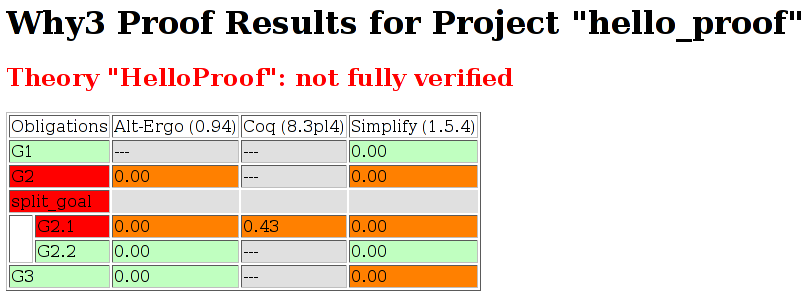
\includegraphics[width=\textwidth]{hello_proof.png}
  \end{center}
  \caption{HTML table produced for the HelloProof example}
\label{fig:html}
\end{figure}

The style 'table' outputs the contents of the session as a table,
similar to the LaTeX output above. Figure~\ref{fig:html} is the HTML table
produced for the 'HelloProof' example, as typically shown in a Web
browser.

The style ''simple' use only 'ul' and 'il' tag. 'jstree' use the 'jstree' plugin
of the javascript library 'jquery'.

\todo{Detailler}


Specific options for this command are as follows.
\begin{description}
\item[\texttt{-o}] 
the directory to output the produces files ('-' for stdout)

\item[\texttt{--context}] adds context around the generated code in
  order to allow direct visualisation (header, css, ...). It also adds
  in the directory all the needed external files. It can't be set with
  stdout output.

\item[\texttt{--style <s>}] sets the style to
  use, among \texttt{simpletree}, \texttt{jstree} and \texttt{table}, defaults to \texttt{table}.

\item[\texttt{--add\_pp <suffix> <cmd> <out\_suffix>}] adds for the
  given prefix the given pretty-printer, the new file as the given
  out\_suffix. cmd must contain
  '\%i' which will be replaced by the input file
                         and '\%o' which will be replaced by the
                         output file.

\item[\texttt{--coqdoc}] use the coqdoc command to display Coq proof
  scripts. This is equivalent to \texttt{--add\_pp .v "coqdoc
    --no-index --html -o \%o \%i" .html}

\end{description}
 
\subsection{Commands modifying the proof attempts}

The subcommands \texttt{mod}, \texttt{copy}, and \texttt{rm} share the
same set of options for selecting the proof attempts to work on:
\begin{itemize}
\item Option \verb|--filter-prover| selects only the proof attempt with
  the given prover. This option can be specified multiple times to
  allow to select all the proofs that corresponds to one of the given
  provers. If this option is not specified, the proof are simply not
  filtered by there corresponding prover.
\item Option \verb|--filter-verified yes| restricts the selection to
  the proofs that are valid and not obsoletes. On contrary the option
  \verb|--filter-verified no| select the ones that are not verified.
  \verb|--filter-verified all|, the default, does not select on this property.
\item Option \verb|--filter-verified-goal yes| restricts the selection
  to the proofs of verified goals (that does not mean that the proof is
  verified). Same for the other cases \verb|no| and \verb|all|.
\item Option \verb|--filter-archived yes| restricts the selection
  to the proofs that are archived. Same for the other cases \verb|no|
  and \verb|all| except the default is \verb|no|.
\end{itemize}

\noindent
The subcommand \texttt{mod} modifies properties of proof
attempts:
\begin{itemize}
\item Option \verb|--set-obsolete| marks the selected proofs as
  obsolete.
\item Option \verb|--set-archived| marks the selected proofs as archived.
\item Option \verb|--unset-archived| removes the archived mark from the selected proofs.
\end{itemize}

The subcommand \texttt{copy} copies the proof attempt of a given goal to another
prover. The new prover is specified by the option
\verb|--to-prover|, for example \texttt{-{}-to-prover Alt-Ergo,0.94}.
A conflict arises if a proof with this prover already exists.
You can choose between four behaviors of \texttt{why3session}:
\begin{itemize}
\item replace the proof (\verb|-f|, \verb|--force|);
\item do not replace thr proof (\verb|-n|, \verb|--never|);
\item replace the proof unless it is verified (valid and not
  obsolete) (\verb|-c|, \verb|--conservative|); this is the default;
\item ask the user each time the case arises (\verb|-i|, \verb|--interactive|).
\end{itemize}


If you just want to update one session with updated provers you can
use \verb|--convert-unknown| instead of the option \verb|--to-prover|.
\begin{verbatim}
why3session copy  --convert-unknown
\end{verbatim}
For each proof attempt associated to an unknown prover (a prover not in
\verb|.why3.conf|) and not archived, it will try to find a known prover
with the same name. If it finds one, the proof attempt is copied to this
prover and the old proof is set to archived. The corresponding edited
files, if any, are copied and regenerated for the new prover An archived
proof is not replayed by why3replayer.

The subcommand \texttt{rm} removes the selected proof
attempts. The options \verb|-i, --interactive|, \verb|-f, --force| and
\verb|-c, --conservative| can also be used to respectively ask before
each suppression, suppress all the selected proof (default) and remove
only the proof that are not verified. The macro option \verb|--clean|
corresponds to \verb|--filter-verified-goal --conservative| and
removes the proof attempts that are not verified but which correspond
to verified goals.


\section{The \texttt{why3.conf} configuration file}
\label{sec:whyconffile}

\todo{THIS SECTION IS OUTDATED}

\begin{figure}[t]
\begin{verbatim}
[main ]
loadpath = "/usr/local/share/why3/theories"
magic = 2
memlimit = 0
running_provers_max = 2
timelimit = 10

[ide ]
default_editor = "emacs"
task_height = 384
tree_width = 438
verbose = 0
window_height = 779
window_width = 638

[prover coq]
command = "coqc %f"
driver = "/usr/local/share/why3/drivers/coq.drv"
editor = "coqide"
name = "Coq"
version = "8.2pl2"

[prover alt-ergo]
command = "why3-cpulimit %t %m alt-ergo %f"
driver = "/usr/local/share/why3/drivers/alt_ergo.drv"
editor = ""
name = "Alt-Ergo"
version = "0.91"
\end{verbatim}
  \caption{Sample why3.conf file}
\label{fig:why3conf}
\end{figure}



One can use a custom configuration file. \texttt{why3config}
and other \texttt{why3} tools use priorities for which
user's configuration file to consider:
\begin{itemize}
\item the file specified by the \texttt{-C} or \texttt{-{}-config} options,
\item the file specified by the environment variable
  \texttt{WHY3CONFIG} if set.
\item the file \texttt{\$HOME/.why3.conf}
  (\texttt{\$USERPROFILE/.why3.conf} under Windows) or, in the case of
  local installation, \texttt{why3.conf} in Why3 sources top directory.
\end{itemize}
If none of these files exists, a built-in default configuration is used.

The configuration file is a human-readable text file, which consists
of association pairs arranged in sections. Figure~\ref{fig:why3conf}
shows an example of configuration file.

A section begins with a header inside square brackets and ends at the
beginning of the next section. The header of a
section can be only one identifier, \texttt{main} and \texttt{ide} in
the example, or it can be composed by a family name and one family
argument, \texttt{prover} is one family name, \texttt{coq} and
\texttt{alt-ergo} are the family argument.

Inside a section, one key can be associated with an integer (\eg{} -555),
a boolean (true, false) or a string (\eg{} "emacs"). One key can appear
only once except if its a multi-value key. The order of apparition of
the keys inside a section matter only for the multi-value key.

\section{Drivers of External Provers}
\label{sec:drivers}

The drivers of external provers are readable files, in directory
\texttt{drivers}. Experimented users can modify them to change the way
the external provers are called, in particular which transformations
are applied to goals.

[TO BE COMPLETED LATER]

\section{Transformations}
\label{sec:transformations}

Here is a quick documentation of provided transformations. We give
first the non-splitting ones, \eg{} those which produce one goal as
result, and others which produces any number of goals.

Notice that the set of available transformations in your own
installation is given by
\begin{verbatim}
why3 --list-transforms
\end{verbatim}

\subsection{Non-splitting transformations}

\begin{description}

\item[eliminate\_algebraic] Replaces algebraic data types by first-order
definitions~\cite{paskevich09rr}

\item[eliminate\_builtin] Suppress definitions of symbols which are
  declared as builtin in the driver, i.e. with a ``syntax'' rule.
\item[eliminate\_definition\_func]
  Replaces all function definitions with axioms.
\item[eliminate\_definition\_pred]
  Replaces all predicate definitions with axioms.
\item[eliminate\_definition]
  Apply both transformations above.
\item[eliminate\_mutual\_recursion]
  Replaces mutually recursive definitions with axioms.
\item[eliminate\_recursion]
  Replaces all recursive definitions with axioms.

\item[eliminate\_if\_term] replaces terms of the form \texttt{if
    formula then t2 else t3} by lifting them at the level of formulas.
  This may introduce \texttt{if then else } in formulas.

\item[eliminate\_if\_fmla] replaces formulas of the form \texttt{if f1 then f2
  else f3} by an equivalent formula using implications and other
  connectives.

\item[eliminate\_if]
  Apply both transformations above.

\item[eliminate\_inductive] replaces inductive predicates by
  (incomplete) axiomatic definitions, i.e. construction axioms and
  an inversion axiom.

\item[eliminate\_let\_fmla]
  Eliminates \texttt{let} by substitution, at the predicate level.

\item[eliminate\_let\_term]
  Eliminates \texttt{let} by substitution, at the term level.

\item[eliminate\_let]
  Apply both transformations above.

% \item[encoding\_decorate\_mono]

% \item[encoding\_enumeration]

\item[encoding\_smt]
  Encode polymorphic types into monomorphic type~\cite{conchon08smt}.

\item[encoding\_tptp]
  Encode theories into unsorted logic. %~\cite{cruanes10}.

% \item[filter\_trigger] *)

% \item[filter\_trigger\_builtin] *)

% \item[filter\_trigger\_no\_predicate] *)

% \item[hypothesis\_selection] *)
%   Filter hypothesis of goals~\cite{couchot07ftp,cruanes10}. *)

\item[inline\_all]
  expands all non-recursive definitions.

\item[inline\_goal] Expands all outermost symbols of the goal that
  have a non-recursive definition.

\item[inline\_trivial]
  removes definitions of the form

\begin{verbatim}
function  f x_1 .. x_n = (g e_1 .. e_k)
predicate p x_1 .. x_n = (q e_1 .. e_k)
\end{verbatim}
when each $e_i$ is either a ground term or one of the $x_j$, and
each $x_1$ .. $x_n$ occur at most once in the $e_i$

\item[introduce\_premises] moves antecedents of implications and
  universal quantifications of the goal into the premises of the task.

% \item[remove\_triggers] *)
%   removes the triggers in all quantifications. *)

\item[simplify\_array] Automatically rewrites the task using the lemma
  \verb|Select_eq| of theory \verb|array.Array|.

\item[simplify\_formula] reduces trivial equalities $t=t$ to true and
  then simplifies propositional structure: removes true, false, ``f
  and f'' to ``f'', etc.

\item[simplify\_recursive\_definition] reduces mutually recursive
  definitions if they are not really mutually recursive, e.g.:
\begin{verbatim}
function f : ... = .... g ...

with g : .. = e
\end{verbatim}
becomes
\begin{verbatim}
function g : .. = e
function f : ... = .... g ...
\end{verbatim}
if f does not occur in e

\item[simplify\_trivial\_quantification]
  simplifies quantifications of the form
\begin{verbatim}
  forall x, x=t -> P(x)
\end{verbatim}
or
\begin{verbatim}
  forall x, t=x -> P(x)
\end{verbatim}
  when x does not occur in t
  into
\begin{verbatim}
P(t)
\end{verbatim}
  More generally, it applies this simplification whenever x=t appear
  in a negative position.

\item[simplify\_trivial\_quantification\_in\_goal]
  same as above but applies only in the goal.

\item[split\_premise]
  splits conjunctive premises.

\end{description}

\subsection{Splitting transformations}

\begin{description}

\item[full\_split\_all]
  composition of \texttt{split\_premise} and \texttt{full\_split\_goal}.

\item[full\_split\_goal] puts the goal in a conjunctive form,
  returns the corresponding set of subgoals. The number of subgoals
  generated may be exponential in the size of the initial goal.

\item[simplify\_formula\_and\_task] same as \texttt{simplify\_formula}
  but also removes the goal if it is equivalent to true.

\item[split\_all]
  composition of \texttt{split\_premise} and \texttt{split\_goal}.

\item[split\_goal] if the goal is a conjunction of goals, returns the
  corresponding set of subgoals. The number of subgoals generated is linear in
  the size of the initial goal.

\item[split\_intro]
  when a goal is an implication, moves the antecedents into the premises.

\end{description}



%%% Local Variables:
%%% mode: latex
%%% TeX-PDF-mode: t
%%% TeX-master: "manual"
%%% End:
